\chapter{Implementation} \label{sec:ch_implementation}


%%%%%%%%%%%%%%%%%%%%%%%%%%%%%%%%%%%%%%%%%%%%%%%%%%%%%%%%%%%%%%%%%%%%%%%%%%%%%%%%%%%%%
%%%%%%%%%%%%%%%%%%%%%%%%%%%%%%%%%%%%%%%%%%%%%%%%%%%%%%%%%%%%%%%%%%%%%%%%%%%%%%%%%%%%%
\section{Manual Design of Extraction Rules} \label{sec:impl_manual_rules}


\subsection{Procedural Extraction Rules} \label{sec:ch50_Procedural_Extraction_Rules} \label{sec:impl_btred_rules}

Our first extraction method, which is based on procedural extraction rules, was implemented using Btred\footnote{See details about Btred in Section~\ref{sec:third_tred}.} API for processing linguistic trees. The extraction rules were implemented in Perl as Btred procedures. Application of these extraction rules on a corpus of linguistic trees is realized such that each procedure (or extraction rule) is executed on every available tree by Btred. 

An example of such extraction rule is in Figure~\ref{lst:btred_rule} and corresponding extraction output on Figure~\ref{fig:btred_xml}. TODO: explain


%%%%%%%%%%%%%%%%%%%%%%%%%%%%%%%%%%%%%%%%%%%%%%%%%%%%%%%%%%%%%%%%%%%%%%%%%%%%%%%%%%%%%
\begin{figure}
\begin{minted}[linenos,  fontsize=\footnotesize,
               frame=lines]{perl}
#variable $this contains currently processed node, $root current root node

my @injure_verbs = ("zranit", "usmrtit", "zemřít", "zahynout", "přežít");

sub print_injured {
	if ($this->{gram}{sempos} eq "v") {
		foreach my $v (@injure_verbs) {
			if ($this->{t_lemma} eq $v ) {
				#action type
				print "<action type=\"" . $this->{t_lemma} . "\">";

				#sentece
				print "<sentece>" . PML_T::GetSentenceString($root) . "</sentece>";
				print "<sentece_id>" . $root->{id} . "</sentece_id>";
				
				#negation
				if (test_negation($this)) {
					print "<negation>true</negation>" ;					
				} else {
					print "<negation>false</negation>" ;										
				}
								
				#manner of injurance
				my @mans = find_node_by_attr_depth($this, 0, 'functor', '^MANN');
				if (@mans) {
					foreach my $m (@mans) {
						print "<manner>"; 
						print $m->{t_lemma};
						print "</manner>"; 
					};
				}
				
				#actors and patients
				my @pats = find_node_by_attr($this, 'functor', '^[PA][AC]T');
				@pats = &filter_list(\&test_person, @pats);
				
				foreach my $p (@pats) {
					print "<participant type=\"" . $p->{t_lemma} . "\">";

					#patients count
					my @cnt = find_node_by_attr($p, 'functor', '^RSTR');
					@cnt = &filter_list(\&test_number_lemma, @cnt);
					my $cnt1 = pop(@cnt);
					print "<quantity>" . 
						&test_number($cnt1->{t_lemma}) . 
						"</quantity>" if ($cnt1);
	
					print "<full_string>";
					print_subtree_as_text($p);
					print "</full_string>";

					print "</participant>";
				}
				
				#action end
				print "</action>\n";											
}}}}
\end{minted} 
																																		\begin{comment}
																																		this >>$<< hacks my syntax highlighter :-)
																																		\end{comment}
\caption{Procedurally written extraction rule in \emph{Btred}.}
\label{lst:btred_rule}
\end{figure}
%%%%%%%%%%%%%%%%%%%%%%%%%%%%%%%%%%%%%%%%%%%%%%%%%%%%%%%%%%%%%%%%%%%%%%%%%%%%%%%%%%%%%




%%%%%%%%%%%%%%%%%%%%%%%%%%%%%%%%%%%%%%%%%%%%%%%%%%%%%%%%%%%%%%%%%%%%%%%%%%%%%%%%%%%%%
\begin{figure}
\begin{minted}[linenos,  fontsize=\footnotesize,
               frame=lines]{xml}
<injured_result>
	<action type="zranit">
		<sentece>
			Při požáru byla jedna osoba lehce zraněna -- jednalo se
			o majitele domu, který si vykloubil rameno.
		</sentece>
		<sentece_id>T-vysocina63466.txt-001-p1s4</sentece_id>
		<negation>false</negation>
		<manner>lehký</manner>
		<participant type="osoba">
			<quantity>1</quantity>
			<full_string>jedna osoba</full_string>
		</participant>
	</action>
	<action type="zemřít">
		<sentece>
			Ve zdemolovaném trabantu na místě zemřeli dva muži -- 82letý
			senior a další muž, jehož totožnost zjišťují policisté.
		</sentece>
		<sentece_id>T-jihomoravsky49640.txt-001-p1s4</sentece_id>
		<negation>false</negation>
		<participant type="muž">
			<quantity>2</quantity>
			<full_string>dva muži</full_string>
		</participant>
	</action>
		<action type="zranit">
		<sentece>čtyřiatřicetiletý řidič nebyl zraněn.</sentece>
		<sentece_id>T-jihomoravsky49736.txt-001-p4s3</sentece_id>
		<negation>true</negation>
		<participant type="řidič">
			<full_string>čtyřiatřicetiletý řidič</full_string>
		</participant>
	</action>
</injured_result>
\end{minted}
\caption{\emph{XML} structured output of the query written in \emph{Btred}.}
\label{fig:btred_xml}
\end{figure}
%%%%%%%%%%%%%%%%%%%%%%%%%%%%%%%%%%%%%%%%%%%%%%%%%%%%%%%%%%%%%%%%%%%%%%%%%%%%%%%%%%%%%





\subsection{Netgraph Based Extraction Rules} \label{sec:ch50_Netgraph_Based_Extraction_Rules}

Our second extraction method, which is based on Netgraph (see Section~\ref{sec:ch30_netgraph} for details), is implemented in Java. Java was chosen partly because we use the Java implementation of Netgraph client as a library. 



The extraction is implemented as follows: Netgraph implementation is responsible for the evaluation of the Netgraph query part of extraction rules and matching trees are then returned to our implementation, which prepares the extraction output based on the SELECT part of extraction rules.




\begin{figure}
	\centering
		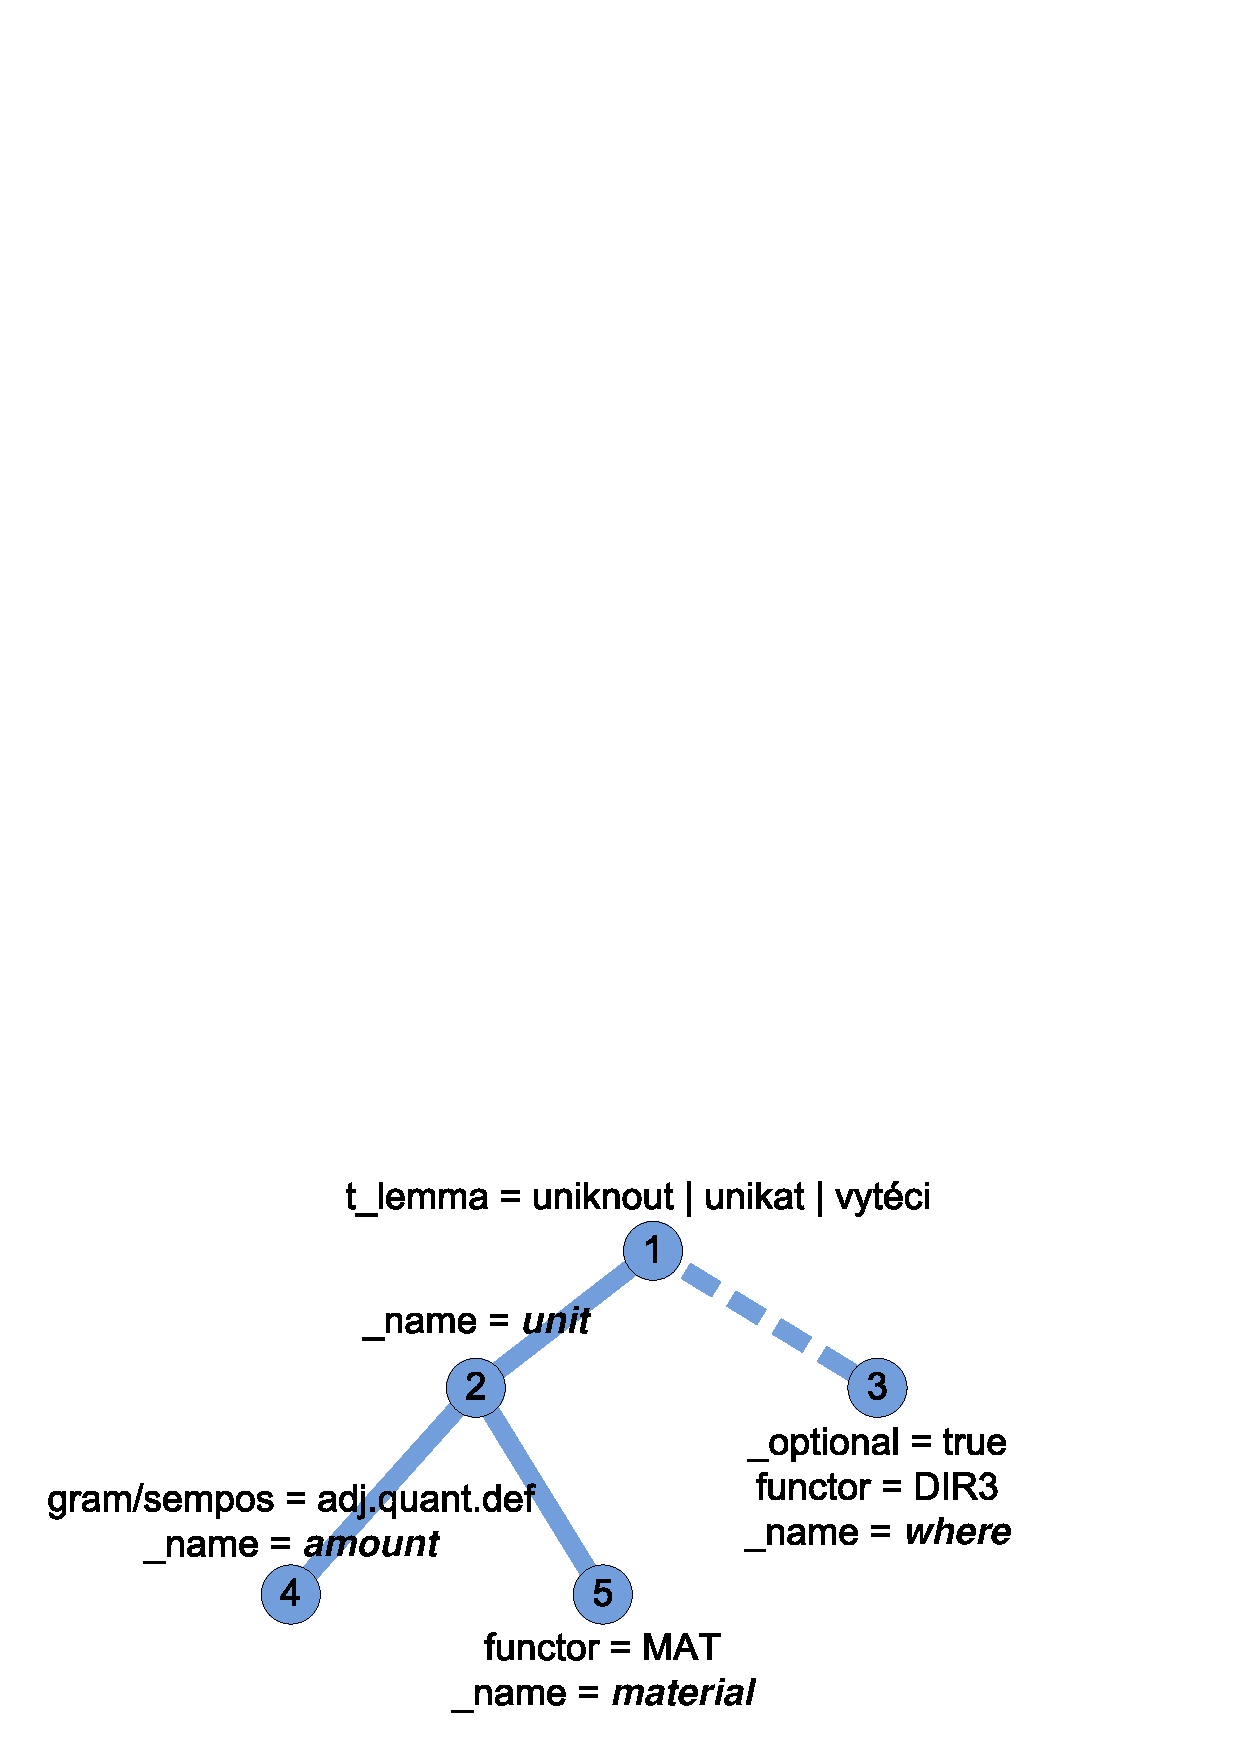
\includegraphics[width=0.5\hsize]{eenv_extract_patern}
\\Transcript:\\
\begin{tabular}{|c|c|}
\hline
uniknout, unikat & vytéci\\
to leak out & to flow out\\
\hline
\end{tabular}		
	\caption{A manually created extraction rule investigating dangerous liquids that spilled out into the environment.}
	\label{fig:ch50_eenv_extract_patern}
\end{figure}


\begin{figure}
	\centering
		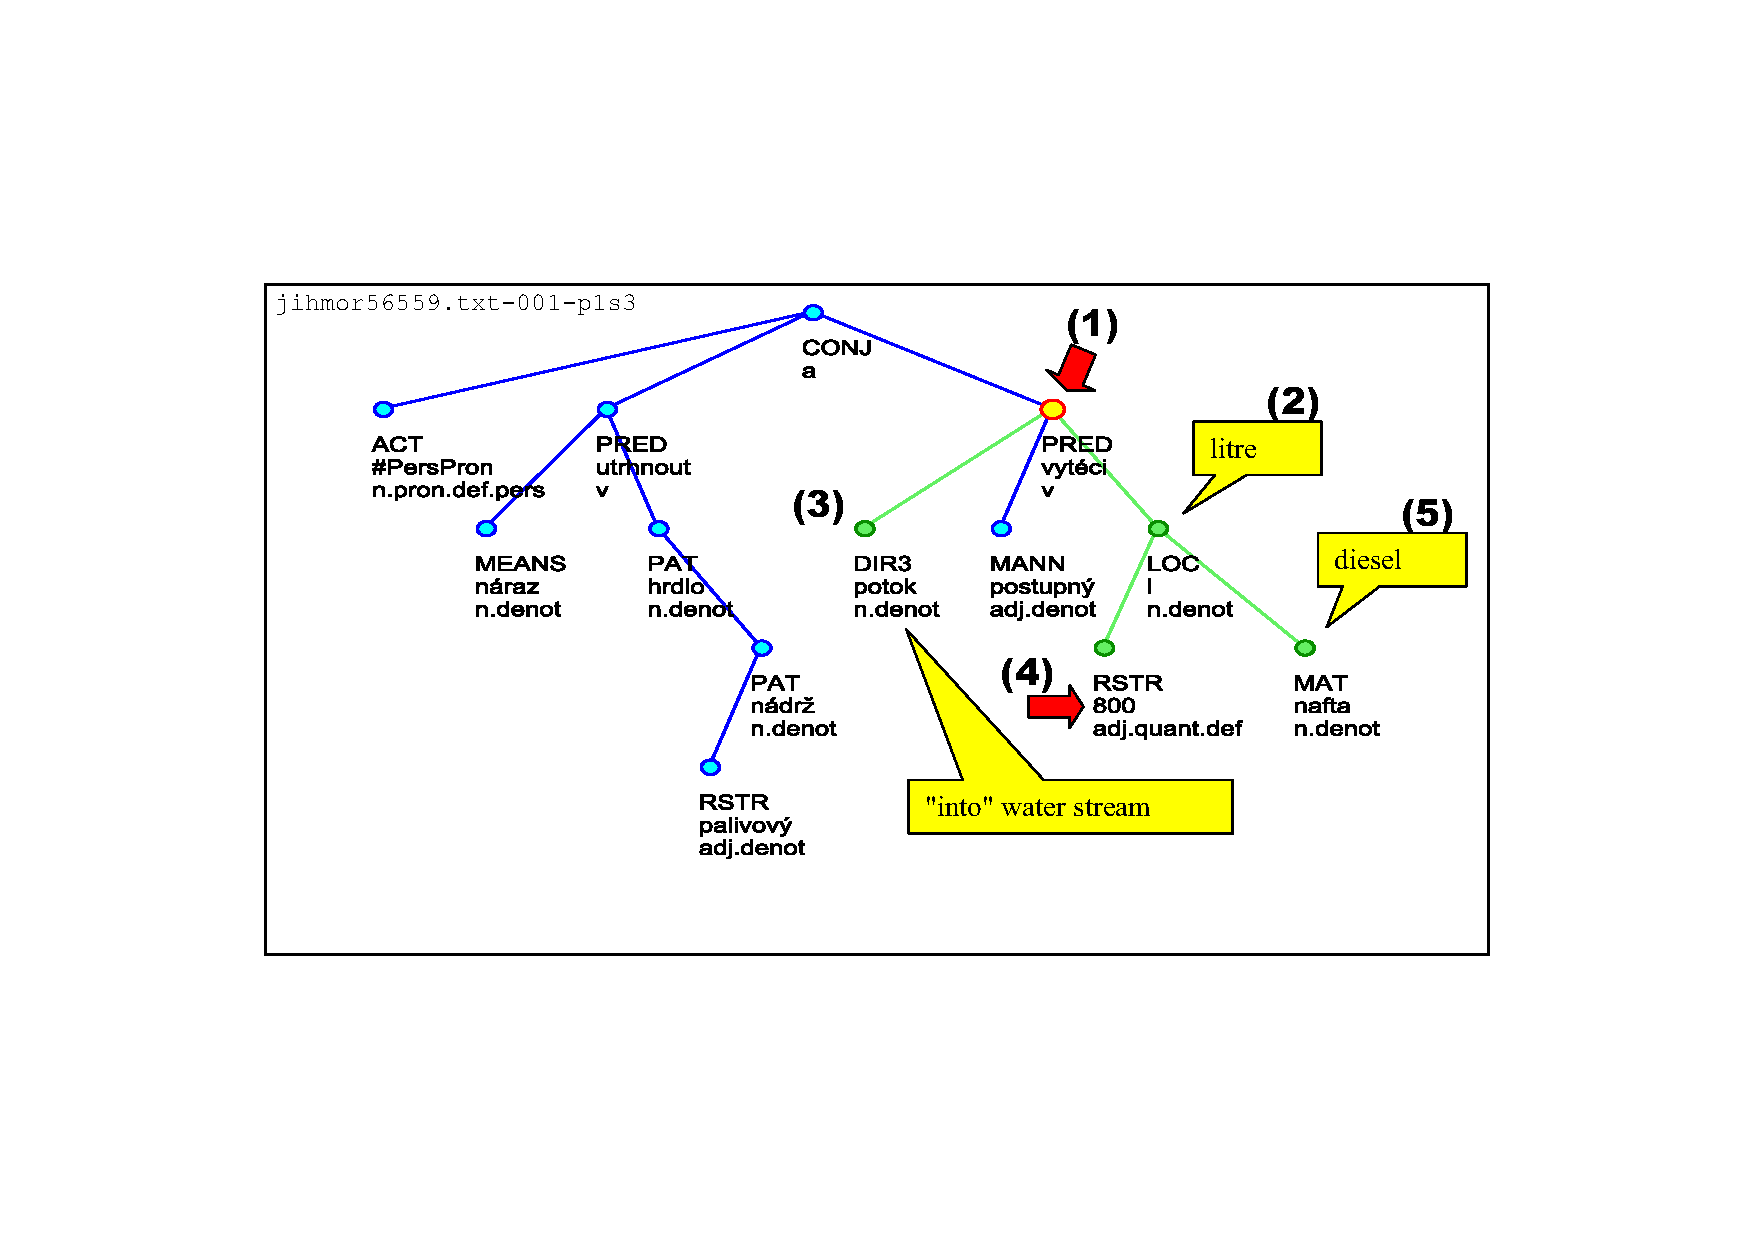
\includegraphics[angle=-90, width=0.6\hsize]{eenv_matching_tree}
		
Original sentence: 
\emph{``Nárazem se utrhl hrdlo palivové nádrže a do potoka postupně vyteklo na 800 litrů nafty.''}\\
English transcript: 
\emph{``Due to the clash the throat of fuel tank tore off and 800 liters of oil (diesel) has run out to a stream.''}
	\caption{A tree matching with the corresponding extraction rule in Figure~\ref{fig:ch50_eenv_extract_patern}.}
	\label{fig:ch50_eenv_matching_tree}
\end{figure}


%%%%%%%%%%%%%%%%%%%%%%%%%%%%%%%%%%%%%%%%%%%%%%%%%%%%%%%%%%%%%%%%%%%%%%%%%%%%%%%%%%%%%
\begin{figure}
\begin{minted}[linenos,  fontsize=\footnotesize,
               frame=lines]{xml}
<QueryMatches>
	<Match root_id="T-vysocina63466.txt-001-p1s4" match_string="2:0,7:3,8:4,11:2">
		<Sentence>
			Při požáru byla jedna osoba lehce zraněna - jednalo se
			o majitele domu, který si vykloubil rameno.
		</Sentence>
		<Data>
			<Value variable_name="action_type" attribute_name="t_lemma">zranit</Value>
			<Value variable_name="injury_manner" attribute_name="t_lemma">lehký</Value>
			<Value variable_name="participant" attribute_name="t_lemma">osoba</Value>
			<Value variable_name="quantity" attribute_name="t_lemma">jeden</Value>
		</Data>
	</Match>
	<Match root_id="T-jihomoravsky49640.txt-001-p1s4" match_string="1:0,13:3,14:4">
		<Sentence>
			Ve zdemolovaném trabantu na místě zemřeli dva muži - 82letý senior
			a další muž, jehož totožnost zjišťují policisté.
		</Sentence>
		<Data>
			<Value variable_name="action_type" attribute_name="t_lemma">zemřít</Value>
			<Value variable_name="participant" attribute_name="t_lemma">muž</Value>
			<Value variable_name="quantity" attribute_name="t_lemma">dva</Value>
		</Data>
	</Match>
	<Match root_id="T-jihomoravsky49736.txt-001-p4s3" match_string="1:0,3:3,7:1">
		<Sentence>Čtyřiatřicetiletý řidič nebyl zraněn.</Sentence>
		<Data>
			<Value variable_name="action_type" attribute_name="t_lemma">zranit</Value>
			<Value variable_name="a-negation" 
			       attribute_name="m/tag">VpYS---XR-NA---</Value>
			<Value variable_name="participant" attribute_name="t_lemma">řidič</Value>
		</Data>
	</Match>
</QueryMatches>
\end{minted}
\caption{\emph{XML} structured output of the SQL select like query. A negation can be detected from the presence of \emph{m/tag} on the line 30.}
\label{fig:select_xml}
\end{figure}
%%%%%%%%%%%%%%%%%%%%%%%%%%%%%%%%%%%%%%%%%%%%%%%%%%%%%%%%%%%%%%%%%%%%%%%%%%%%%%%%%%%%%

\begin{figure}
	\centering
		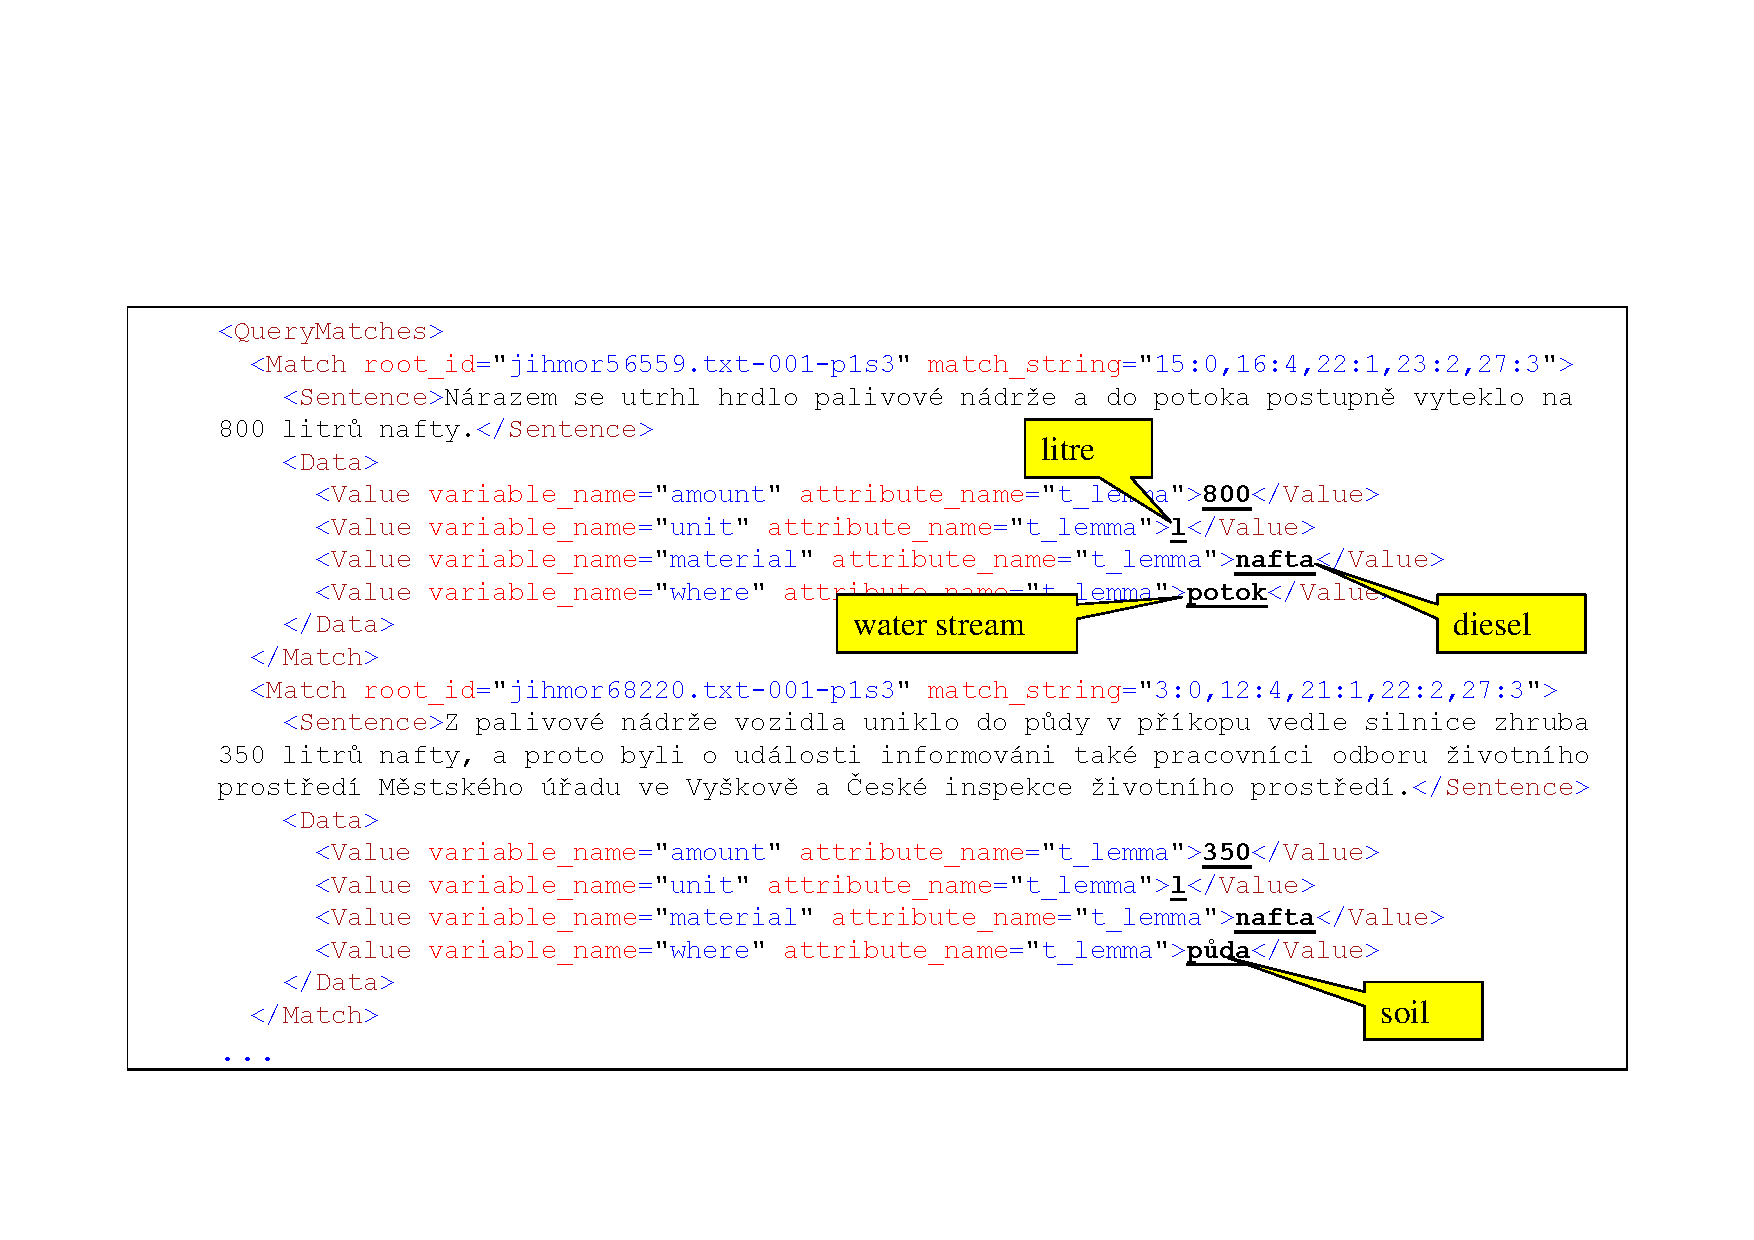
\includegraphics[angle=-90, width=0.7\hsize]{eenv_results}
	\caption{\emph{XML} structured output of the SQL select like query corresponding with the extraction rule in Figure~\ref{fig:ch50_eenv_extract_patern} and matching tree in Figure~\ref{fig:ch50_eenv_matching_tree}.}
	\label{fig:ch50_eenv_results}
\end{figure}























\subsubsection{Illustration Examples}



Evaluation of the extraction rule from Figure~\ref{fig:ch50_eenv_extract_patern} is illustrated on Figure~\ref{fig:ch50_eenv_matching_tree}. Figure~\ref{fig:ch50_eenv_matching_tree} shows a linguistic tree matching with the extraction rule. Matching nodes are decorated and labeled by the numbers of corresponding query nodes.



\subsection{Extraction Output} \label{sec:impl_manual_output}

Small pieces of extraction outputs are shown in Figure~\ref{fig:select_xml} (for the extraction rule in Figure~\ref{fig:ch50_extract_patern}) and in Figure~\ref{fig:ch50_eenv_results} (for the extraction rule in Figure~\ref{fig:ch50_eenv_extract_patern}). 

The former example (Figure~\ref{fig:select_xml}) contains three matches of the extraction rule in three different articles. Each query match is closed in the \verb+<Match>+ element and each contains values of some linguistic attributes closed inside the \verb+<Value>+ elements. Each value comes from some of the nodes of the extraction rule. Name of corresponding query node is saved in the \verb+variable_name+ attribute of the \verb+<Value>+ element.

In the case of the example query, values identified by the variable \verb+action_type+ specify the type of the action. So in the first and third case somebody was injured (\emph{zranit} means to injure in Czech, lines 8 and 28) and in the second case somebody died (\emph{zemřít} means to die in Czech, line 20).

Values identified by \verb+participant+ and \verb+quantity+ contain information about participants of the action. \verb+participant+ serves for specification of the type of the participants and \verb+quantity+ values hold numbers (quantity) of the participants. So in the first action one (\emph{jeden}, line 11) person (\emph{osoba}, line 10) was injured and in the second action two (\emph{dva}, line 22) men (\emph{muž}, line 21) died.

Values identified by \verb+a-negation+ contain the information about a negation of a clause (The presence of negation is indicated by the 11th character of the position-based morphological tag, note that the corresponding node (number 2) of the extraction rule is marked as optional and the restriction on m/tag is put in the form of regular expression on the 11th character.) So we can see that the participant (driver -- \emph{řidič}, line 31) of the last action was \textbf{not} injured (lines 29-30).

The last not described attribute name is \verb+injury_manner+. Corresponding values contain information about the manner of injury of an injury action. So in the first action of the example there was a light injury (\emph{lehký} means light in Czech, line 9).








%%%%%%%%%%%%%%%%%%%%%%%%%%%%%%%%%%%%%%%%%%%%%%%%%%%%%%%%%%%%%%%%%%%%%%%%%%%%%%%%%%%%%
%%%%%%%%%%%%%%%%%%%%%%%%%%%%%%%%%%%%%%%%%%%%%%%%%%%%%%%%%%%%%%%%%%%%%%%%%%%%%%%%%%%%%
\section{Machine Learning of Extraction Rules}

\section{Shareable Extraction Ontologies}

\subsection{Data Transformation}

\subsection{Rule Transformations}

\section{Fuzzy ILP Classification}

\subsection{Translation of Fuzzy ILP Task to Several Classical ILP Tasks}

\subsection{Learned Rules Examples}
